\documentclass[conference]{IEEEtran}
\usepackage{graphicx,booktabs,amsmath,cite,url,xcolor}
\graphicspath{{../results/}}
\definecolor{navy}{RGB}{20,50,100}

\begin{document}

% ------------------------------------------------------------ cover page
\begin{titlepage}
\centering
\vspace*{0.5cm}
{\color{navy}\rule{\textwidth}{2.5pt}}\par
\vspace{0.4cm}
{\Large\textsc{Military Institute of Science and Technology}\par}
\vspace{0.1cm}
{\large Department of Computer Science and Engineering\par}
\vspace{0.4cm}
{\color{navy}\rule{\textwidth}{0.6pt}}\par

\vspace{1.8cm}
{\large\textsc{CSE-307: Operating Systems}\par}
\vspace{0.1cm}
{\large Term Paper\par}

\vspace{1.4cm}
{\fontsize{27}{33}\selectfont\bfseries\color{navy} Choosing a Disk Scheduling\\[2pt] Algorithm with a\\[2pt] Decision Tree\par}

\vspace{0.9cm}
{\large\itshape Track 2: Disk Scheduling\par}
\vspace{0.1cm}
{\normalsize\itshape Learning-Augmented OS Heuristics:\\ Classical Algorithms Meet Adaptive Prediction\par}

\vfill
\begin{tabular}{@{}p{0.45\textwidth}@{}p{0.45\textwidth}@{}}
\textbf{\color{navy}Submitted by} & \textbf{\color{navy}Submitted to}\\[4pt]
Anirudha Das & Khaled Hasan Irfan\\
ID: 202414098 & Lecturer\\
 & Department of CSE, MIST\\
\end{tabular}

\vspace{1.6cm}
\fbox{\begin{minipage}{0.8\textwidth}\centering\vspace{3pt}
\textbf{Source code, results and figures}\\[3pt]
\url{https://github.com/Ctfdrim/OS-Term-Paper}\vspace{3pt}
\end{minipage}}

\vspace{1.2cm}
{\large October 2026\par}
\vspace{0.4cm}
{\color{navy}\rule{\textwidth}{2.5pt}}\par
\end{titlepage}

% ------------------------------------------------------------ paper
\title{Choosing a Disk Scheduling Algorithm with a Decision Tree}

\author{\vspace{-3em}}

\maketitle

\begin{abstract}
No disk scheduling algorithm is the best choice for every kind of workload, and the workload on a real machine keeps changing. In this paper I implement FCFS, SCAN, C-SCAN and SSTF and train a small decision tree that looks at a short window of pending requests and predicts which of the four will need the least head movement, together with a confidence score. I test it on synthetic sequential, random and bursty workloads, including timelines where the workload type changes three times. Over ten timelines the selector needs 64.1 thousand tracks of seek per timeline, compared with 65.1 for the best fixed algorithm (SSTF) and 63.0 for an oracle that always picks the best one. Its confidence is higher when it is right (0.90 against 0.64) and is close to its real accuracy. I ran everything on Linux, and I also relate the seek times to virtual memory, because a page fault is a disk read.
\end{abstract}

\section{Introduction}
When a process touches a page that is not in memory, the OS has to bring it in from the backing store, which means a disk read~\cite{silberschatz}. If $p$ is the fraction of memory accesses that cause a page fault, the effective access time is
\begin{equation}
\mathrm{EAT} = (1-p)\,T_m + p\,T_f ,
\label{eq:eat}
\end{equation}
where $T_m$ is the memory access time and $T_f$ is the time to handle a fault. $T_f$ is mostly disk time: controller overhead, seek, rotational latency and transfer. When many processes fault at the same time, or when the system is thrashing~\cite{denning68}, many requests are waiting for the disk, and the order in which the OS serves them decides how much the head has to seek.

The classic algorithms order the queue differently. FCFS is fair but makes the head jump around, SSTF keeps movement small but can starve far-away requests, and SCAN and C-SCAN sweep across the disk to keep waiting times bounded~\cite{denning67,teorey72,seltzer90}. Which one is best depends on the request pattern, and the pattern changes while the system runs. This is an algorithm selection problem~\cite{rice76}, so I wanted to see if a small learned model can make the choice. I try to answer two questions. First, how much total seek time does the selector save compared with each fixed algorithm, also right after the workload changes? Second, is its confidence score reliable, meaning it is higher when the choice is right?

\section{Method}
\subsection{Disk model and algorithms}
The disk has tracks 0 to 199, and I take seek time to be the distance the head moves, so a request is just a track number. Each algorithm gets the head position and the pending requests and returns the path of the head; the total seek is the sum of the distances along the path. FCFS serves requests in arrival order. SSTF always serves the nearest pending request. SCAN moves toward track 0 serving requests on the way, goes to the end of the disk, turns around and sweeps up to the last request. C-SCAN serves requests only while moving toward track 0, then jumps from track 0 to track 199 and continues downward; the jump is counted as movement. I checked the code on the textbook example~\cite{silberschatz} with head 53 and queue 98, 183, 37, 122, 14, 124, 65, 67, where the totals are 640 (FCFS), 236 (SSTF), 236 (SCAN) and 386 (C-SCAN), and the program reproduces these values.

\subsection{Workloads}
Requests arrive as a Poisson stream and are cut into windows of 100 ms. The requests that arrive in one window are the queue to be scheduled. I generate three kinds of workload, each time with new random parameters: \emph{sequential}, with one to three readers that walk along the disk; \emph{random}, with uniformly random tracks; and \emph{bursty}, with a few bursts per window where 10 to 40 requests cluster around a hot track, with idle gaps between bursts. The head starts every window at a random track, which stands for wherever earlier I/O left it, and which means all algorithms get exactly the same input. Windows have 46 requests on average (38 sequential, 37 random, 73 bursty).

\subsection{The selector}
For each window the decision tree gets six numbers: the number of requests, the spread of the tracks, the average jump between consecutive arrivals, the burstiness of the arrivals (the standard deviation of the gaps divided by their mean~\cite{goh08}), the head position, and the share of requests below the head. The label is the algorithm with the lowest total seek; ties go to FCFS, then SCAN, then C-SCAN, then SSTF. I trained a scikit-learn tree~\cite{sklearn} with depth 6 on 11\,560 windows of all three kinds. The confidence is the probability that the tree gives to its choice~\cite{niculescu05}. A choice counts as optimal if its seek equals the minimum over the four algorithms, ties included.

\subsection{Experiments}
To test a workload change, I built timelines of four phases with 100 windows each: sequential, random, bursty and sequential again. There are ten such timelines (3888 windows), none of them used for training. I compare the selector with the four fixed algorithms and with the oracle, which tries all four and keeps the best for every window. All programs ran on Linux (Ubuntu 26.04 under WSL2, kernel 6.6.87.2, 4 vCPUs, 3.8 GB RAM, Python 3.14.4). A second small program reads 4 KB blocks from a 256 MB file on the Linux disk to compare sequential and random access and a cold and a warm page cache.

\begin{figure*}[t]
\centering
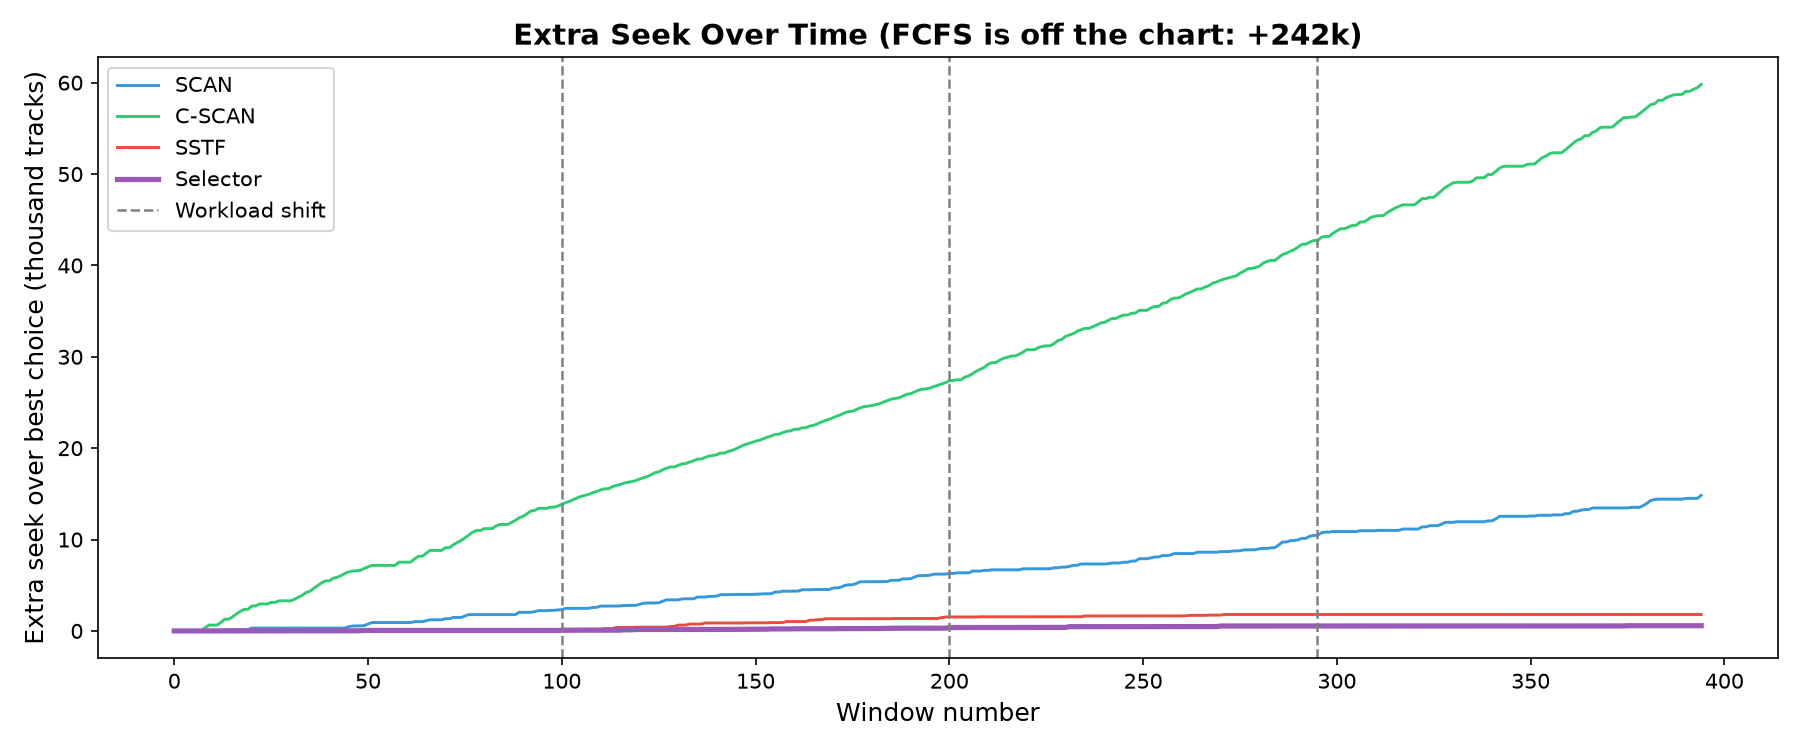
\includegraphics[width=0.9\textwidth]{extra_seek_timeline.png}
\caption{Extra seek over the best choice, added up over one timeline. A flat line means the policy was always as good as the best one. The dashed lines are the workload changes. FCFS is far above the chart.}
\label{fig:timeline}
\end{figure*}

\section{Results}
\subsection{Total seek time}
Table~\ref{tab:seek} shows the seek time of every policy. Over a timeline FCFS needs 528.7 thousand tracks, about eight times as much as SSTF (65.1). SCAN needs 19\% and C-SCAN 85\% more than SSTF. The selector needs 64.1, which is only 1.7\% above the oracle (63.0), while SSTF is 3.4\% above it (Fig.~\ref{fig:timeline}). The selector is better than always using SSTF in 9 of the 10 timelines, with a saving of 1.6\% $\pm$ 0.7\%, and it closes about half of the gap between SSTF and the oracle. The gain comes mostly from the random phase (256 against 272 tracks per window); in the other phases the selector is within two tracks of SSTF. Since SSTF is already close to the best possible when only seek distance counts, the main use of the selector is to avoid bad fixed choices like FCFS and SCAN, and to add a small gain on top.

\begin{table*}[t]
\caption{Seek time of each policy. The total is in thousand tracks per timeline (mean and standard deviation over 10 timelines); the phase columns are the mean seek per window in tracks.}
\label{tab:seek}
\centering\small
\begin{tabular}{@{}lrrrrrrr@{}}
\toprule
Policy & Total & Std & Above best & 1 sequential & 2 random & 3 bursty & 4 sequential \\
\midrule
FCFS & 528.7 & 178.8 & +739.0\% & 1292 & 2501 & 855 & 734 \\
SCAN & 77.5 & 8.2 & +22.9\% & 172 & 286 & 197 & 142 \\
C-SCAN & 120.5 & 8.5 & +91.2\% & 283 & 385 & 315 & 257 \\
SSTF & 65.1 & 6.8 & +3.4\% & 129 & 272 & 157 & 111 \\
Selector & \textbf{64.1} & 6.6 & +1.7\% & 131 & \textbf{256} & 158 & 113 \\
Best possible & 63.0 & 6.3 & 0 & 128 & 254 & 154 & 111 \\
\bottomrule
\end{tabular}
\end{table*}

\subsection{What changes when the workload changes}
No algorithm wins everywhere. SSTF reaches the lowest seek in 99\%, 72\% and 94\% of the sequential, random and bursty windows, and SCAN in 69\%, 42\% and 59\%. FCFS is the best in 19\% of the sequential windows, where a single reader already sends requests in a good order, and never in the others. C-SCAN is only ever best in a tie with SCAN, because once its jump from 0 to 199 is counted, SCAN's path is never longer; its real advantage, more even waiting times, does not show up in total seek.

FCFS suffers the most from a change of pattern. It goes from 855 tracks per window in the bursty phase to 2501 in the random phase, because a random order makes the head jump about a third of the disk (roughly 67 tracks) for every request. SSTF, SCAN and C-SCAN change by at most 2.5 times between phases (Fig.~\ref{fig:phases}).

The selector hardly notices the changes. In the first 10 windows after a change it makes the optimal choice in 88.7\% of the windows, compared with 90.2\% in the rest, and its seek is 1.8\% and 1.7\% above the best. The reason is that it looks at every window on its own and keeps no memory of the past. The tree uses mostly the share of requests below the head (57\% of the importance), the average jump (24\%) and the head position (14\%), and not so much the workload type. So a change of type matters little as long as the windows look like the ones used for training. I did not test windows that are very different from the training data.

\subsection{Confidence}
The selector makes the optimal choice in 90.0\% of the windows. Its mean confidence is 0.90 when the choice is optimal and 0.64 when it is not, and the AUROC for separating the two cases is 0.89. Figure~\ref{fig:confidence} shows the share of optimal choices in each confidence range: the points follow the diagonal closely (expected calibration error 0.026), and the tree is slightly under-confident for confidence values between 0.7 and 0.9 (for example 95\% optimal choices at confidence 0.87). So the confidence can be used to decide when to trust the selector, for example by falling back on SSTF below a confidence of about 0.65.

\begin{figure}[t]
\centering
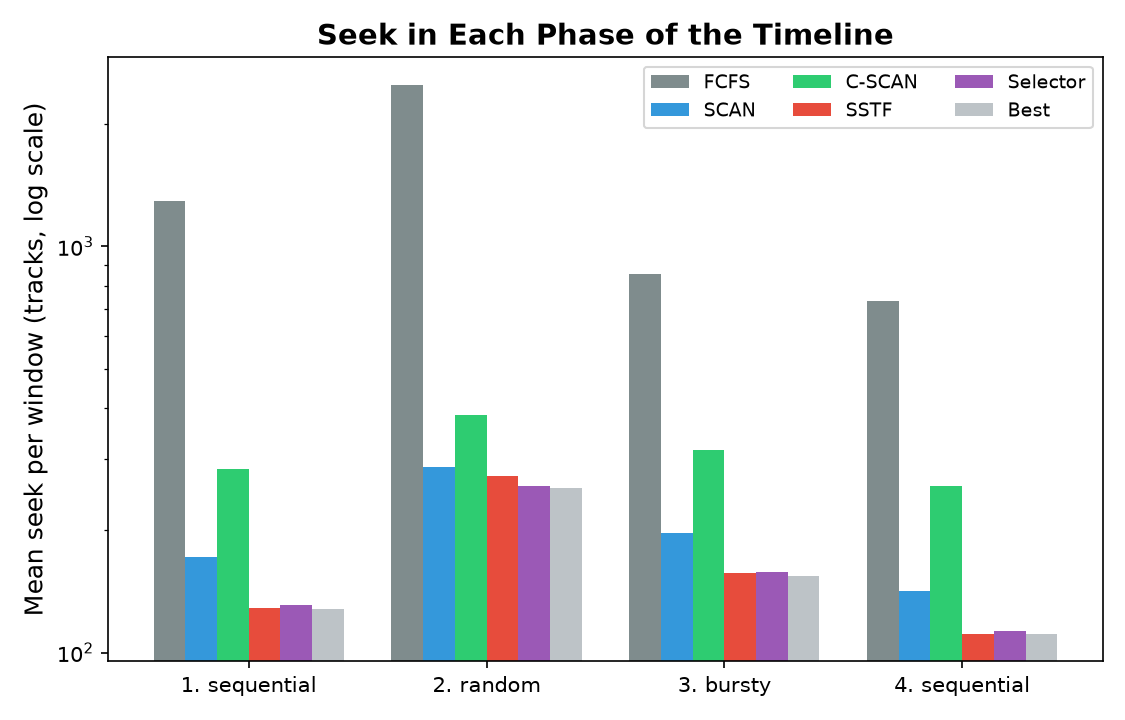
\includegraphics[width=\columnwidth]{seek_by_phase.png}
\caption{Mean seek per window in each phase (log scale).}
\label{fig:phases}
\end{figure}

\begin{figure}[t]
\centering
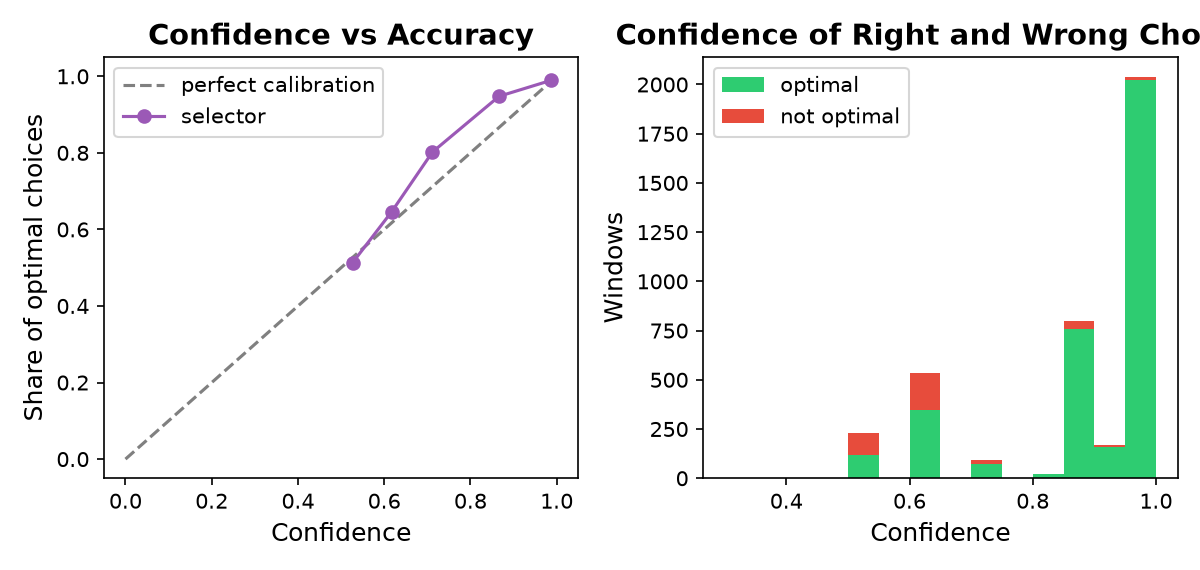
\includegraphics[width=\columnwidth]{confidence.png}
\caption{Left: share of optimal choices for each confidence range. Right: confidence of the optimal and the non-optimal choices.}
\label{fig:confidence}
\end{figure}

\subsection{Effect on virtual memory}
To link the results to paging, I assume that every page fault is one disk request and use Eq.~(\ref{eq:eat}) with $T_m = 100$ ns and a 7200 rpm disk: 0.2 ms controller time, 4.17 ms average rotational latency, 0.03 ms to transfer a 4 KB page and an 8 ms average seek. The average random seek is about 67 tracks, so one track costs about 0.12 ms. With FCFS a request needs 29.5 tracks of seek, so $T_f = 7.94$ ms and the EAT is 894 ns for $p = 10^{-4}$. With the selector a request needs 3.6 tracks, $T_f = 4.83$ ms and the EAT is 583 ns, which is 35\% lower. The saving depends on $p$: it is only 2.9\% at $p = 10^{-6}$, but when the system is thrashing at $p = 10^{-2}$ the EAT is 79.5 $\mu$s with FCFS and 48.4 $\mu$s with the selector, and the saving approaches the 39\% that separates the two fault times. It also requires several faults to be waiting at the same time (here about 46 requests per window); with a single request there is nothing to reorder. Page replacement lowers $p$ and disk scheduling lowers $T_f$, and the two multiply in Eq.~(\ref{eq:eat}).

\subsection{Linux test}
Table~\ref{tab:linux} shows the results of the Linux program. Random 4 KB reads with the page cache bypassed are 37\% slower than sequential ones (27.6 against 43.9 MB/s), so the access pattern matters even on this machine. The page cache matters much more: a read that hits the cache takes 1.1 $\mu$s, a read that misses takes 157 $\mu$s, which is more than 100 times slower. This is the same gap between hit and miss that Eq.~(\ref{eq:eat}) describes for page faults. The Linux disk here is a virtual disk, which hides the real geometry of the platters, so seek time cannot be seen in these numbers. This is why I compared the scheduling algorithms in simulation.

\begin{table}[t]
\caption{Linux test: 20\,000 reads of 4 KB from a 256 MB file, mean $\pm$ std of 5 runs. Direct means the page cache is bypassed.}
\label{tab:linux}
\centering\small
\begin{tabular}{@{}lrr@{}}
\toprule
Test & MB/s & Latency ($\mu$s) \\
\midrule
direct, sequential & 43.9 $\pm$ 3.5 & 93.7 $\pm$ 7.5 \\
direct, random & 27.6 $\pm$ 1.3 & 148.8 $\pm$ 6.8 \\
buffered, cold cache & 26.3 $\pm$ 2.1 & 156.6 $\pm$ 12.7 \\
buffered, warm cache & 3637.6 $\pm$ 471.2 & 1.1 $\pm$ 0.2 \\
\bottomrule
\end{tabular}
\end{table}

\section{Limitations}
Seek time is modelled as distance only, but real seek times are not linear and rotation matters~\cite{ruemmler94}. The windows are independent batches and not an online system, so starvation and waiting-time fairness, which are the main reasons for SCAN and C-SCAN, are not measured. The workloads are synthetic, with parameters that I chose to cover the three kinds, and the confidence is checked on the same kind of data. Ten timelines is a small sample. The Linux numbers come from a virtual disk and change a little from run to run.

\section{Conclusion}
A decision tree with six cheap features picks a disk scheduling algorithm whose total seek is within 1.7\% of the best possible choice. It is better than the best fixed algorithm, SSTF, in 9 of 10 timelines, it is not affected much when the workload type changes, and its confidence score is a reasonable guide to how much to trust it. The gain over SSTF is small, but the gain over FCFS or SCAN is large, and this matters for virtual memory because every page fault is a disk request. The code, the results and the figures are at \url{https://github.com/Ctfdrim/OS-Term-Paper}.

\begin{thebibliography}{99}
\bibitem{silberschatz} A.~Silberschatz, P.~B.~Galvin and G.~Gagne, \emph{Operating System Concepts}, 10th~ed. Wiley, 2018.
\bibitem{denning68} P.~J.~Denning, ``Thrashing: its causes and prevention,'' in \emph{Proc. AFIPS Fall Joint Computer Conf.}, 1968, pp.~915--922.
\bibitem{denning67} P.~J.~Denning, ``Effects of scheduling on file memory operations,'' in \emph{Proc. AFIPS Spring Joint Computer Conf.}, 1967, pp.~9--21.
\bibitem{teorey72} T.~J.~Teorey and T.~B.~Pinkerton, ``A comparative analysis of disk scheduling policies,'' \emph{Commun. ACM}, vol.~15, no.~3, pp.~177--184, 1972.
\bibitem{seltzer90} M.~Seltzer, P.~Chen and J.~Ousterhout, ``Disk scheduling revisited,'' in \emph{Proc. USENIX Winter Technical Conf.}, 1990, pp.~313--324.
\bibitem{rice76} J.~R.~Rice, ``The algorithm selection problem,'' \emph{Advances in Computers}, vol.~15, pp.~65--118, 1976.
\bibitem{goh08} K.-I.~Goh and A.-L.~Barab\'asi, ``Burstiness and memory in complex systems,'' \emph{EPL}, vol.~81, no.~4, p.~48002, 2008.
\bibitem{sklearn} F.~Pedregosa \emph{et al.}, ``Scikit-learn: machine learning in Python,'' \emph{J. Mach. Learn. Res.}, vol.~12, pp.~2825--2830, 2011.
\bibitem{niculescu05} A.~Niculescu-Mizil and R.~Caruana, ``Predicting good probabilities with supervised learning,'' in \emph{Proc. ICML}, 2005, pp.~625--632.
\bibitem{ruemmler94} C.~Ruemmler and J.~Wilkes, ``An introduction to disk drive modeling,'' \emph{IEEE Computer}, vol.~27, no.~3, pp.~17--28, 1994.
\end{thebibliography}

\end{document}
